\section{Introduction}\label{intro}\sloppy
Visual data exploration tools are an important part of exploratory 
data analysis. These tools provide interfaces to interactively explore subsets, summaries, and processing results of their data through visualizations such as bar charts, scatterplots, line charts, and even summary tables.  Visualization is a crucial first-step before formal data modeling and has been widely adopted for understanding machine learning datasets (e.g., Google Facets~\cite{googlefacets}), data preparation (e.g., Trifacta~\cite{trifacta}), business intelligence (e.g., Tableau~\cite{stolte2002polaris}, Spotfire~\cite{shneiderman1999dynamic}), and have increased interest in the database, visualization, and machine learning communities. 

One of the reasons that visualizations are so useful is that analysts can use them to very quickly identify unexpected values, patterns, and trends that would have otherwise been undetected from automated procedures (e.g., the anomaly signatures are subtle or not apriori specified).  Consider the following representative examples from two real-world datasets: 

\begin{example}[Terrorism]
The Global Terrorism Database~\cite{data-terrorism} is a dataset of around terrorist attacks scraped from news sources.  Each record contains the date, location, details about the attack, and the number of fatalities and injuries.  If we plot the number of incidents for each year, we notice a major increase for 2001. While this is partially explained by the occurrence of 9/11 in the United States, the dataset contains a large number of duplicate records for this year due to increased reporting. There are similarly missing years due to date formatting issues.
\label{e:terrorism}
\end{example}

In this example, a histogram can give the analyst broad predicates that might have suspect data, however, to {\it explain} these anomalies, current users must resort to a combination of manual data inspection and programmatic tools. These unexpected values are not due to real anomalous phenomena but also a combination of inconsistencies in the underlying dataset.  This mix between real outliers and data errors requires the analyst to ``context switch'' into data cleaning mode--to write ad-hoc scripts to handle these issues--and then, switch back the analysis mode to continue. For analysts working with a variety of data sources, it is not scalable to perform manual analysis for anomalies encountered in every dataset.

Recent projects have proposed \emph{explanation engines} that automatically search for candidate explanations for user-defined anomalies.  These tools take as input complaint specifications (e.g., whether output attribute values are too high, too low, or otherwise incorrect) and output a ranked list of query predicates most correlated with the anomalies~\cite{scorpion,DBLP:conf/sigmod/ChalamallaIOP14,bailis2016macrobase,roy2015explaining}.  One way of interpreting these predicates is as exclusion rules--i.e., deleting input records that satisfy the predicates help ``resolve'' the user-specified complaints with minimal effects on non-complaint results~\cite{scorpion}.  

\begin{figure}[tb]
\centering
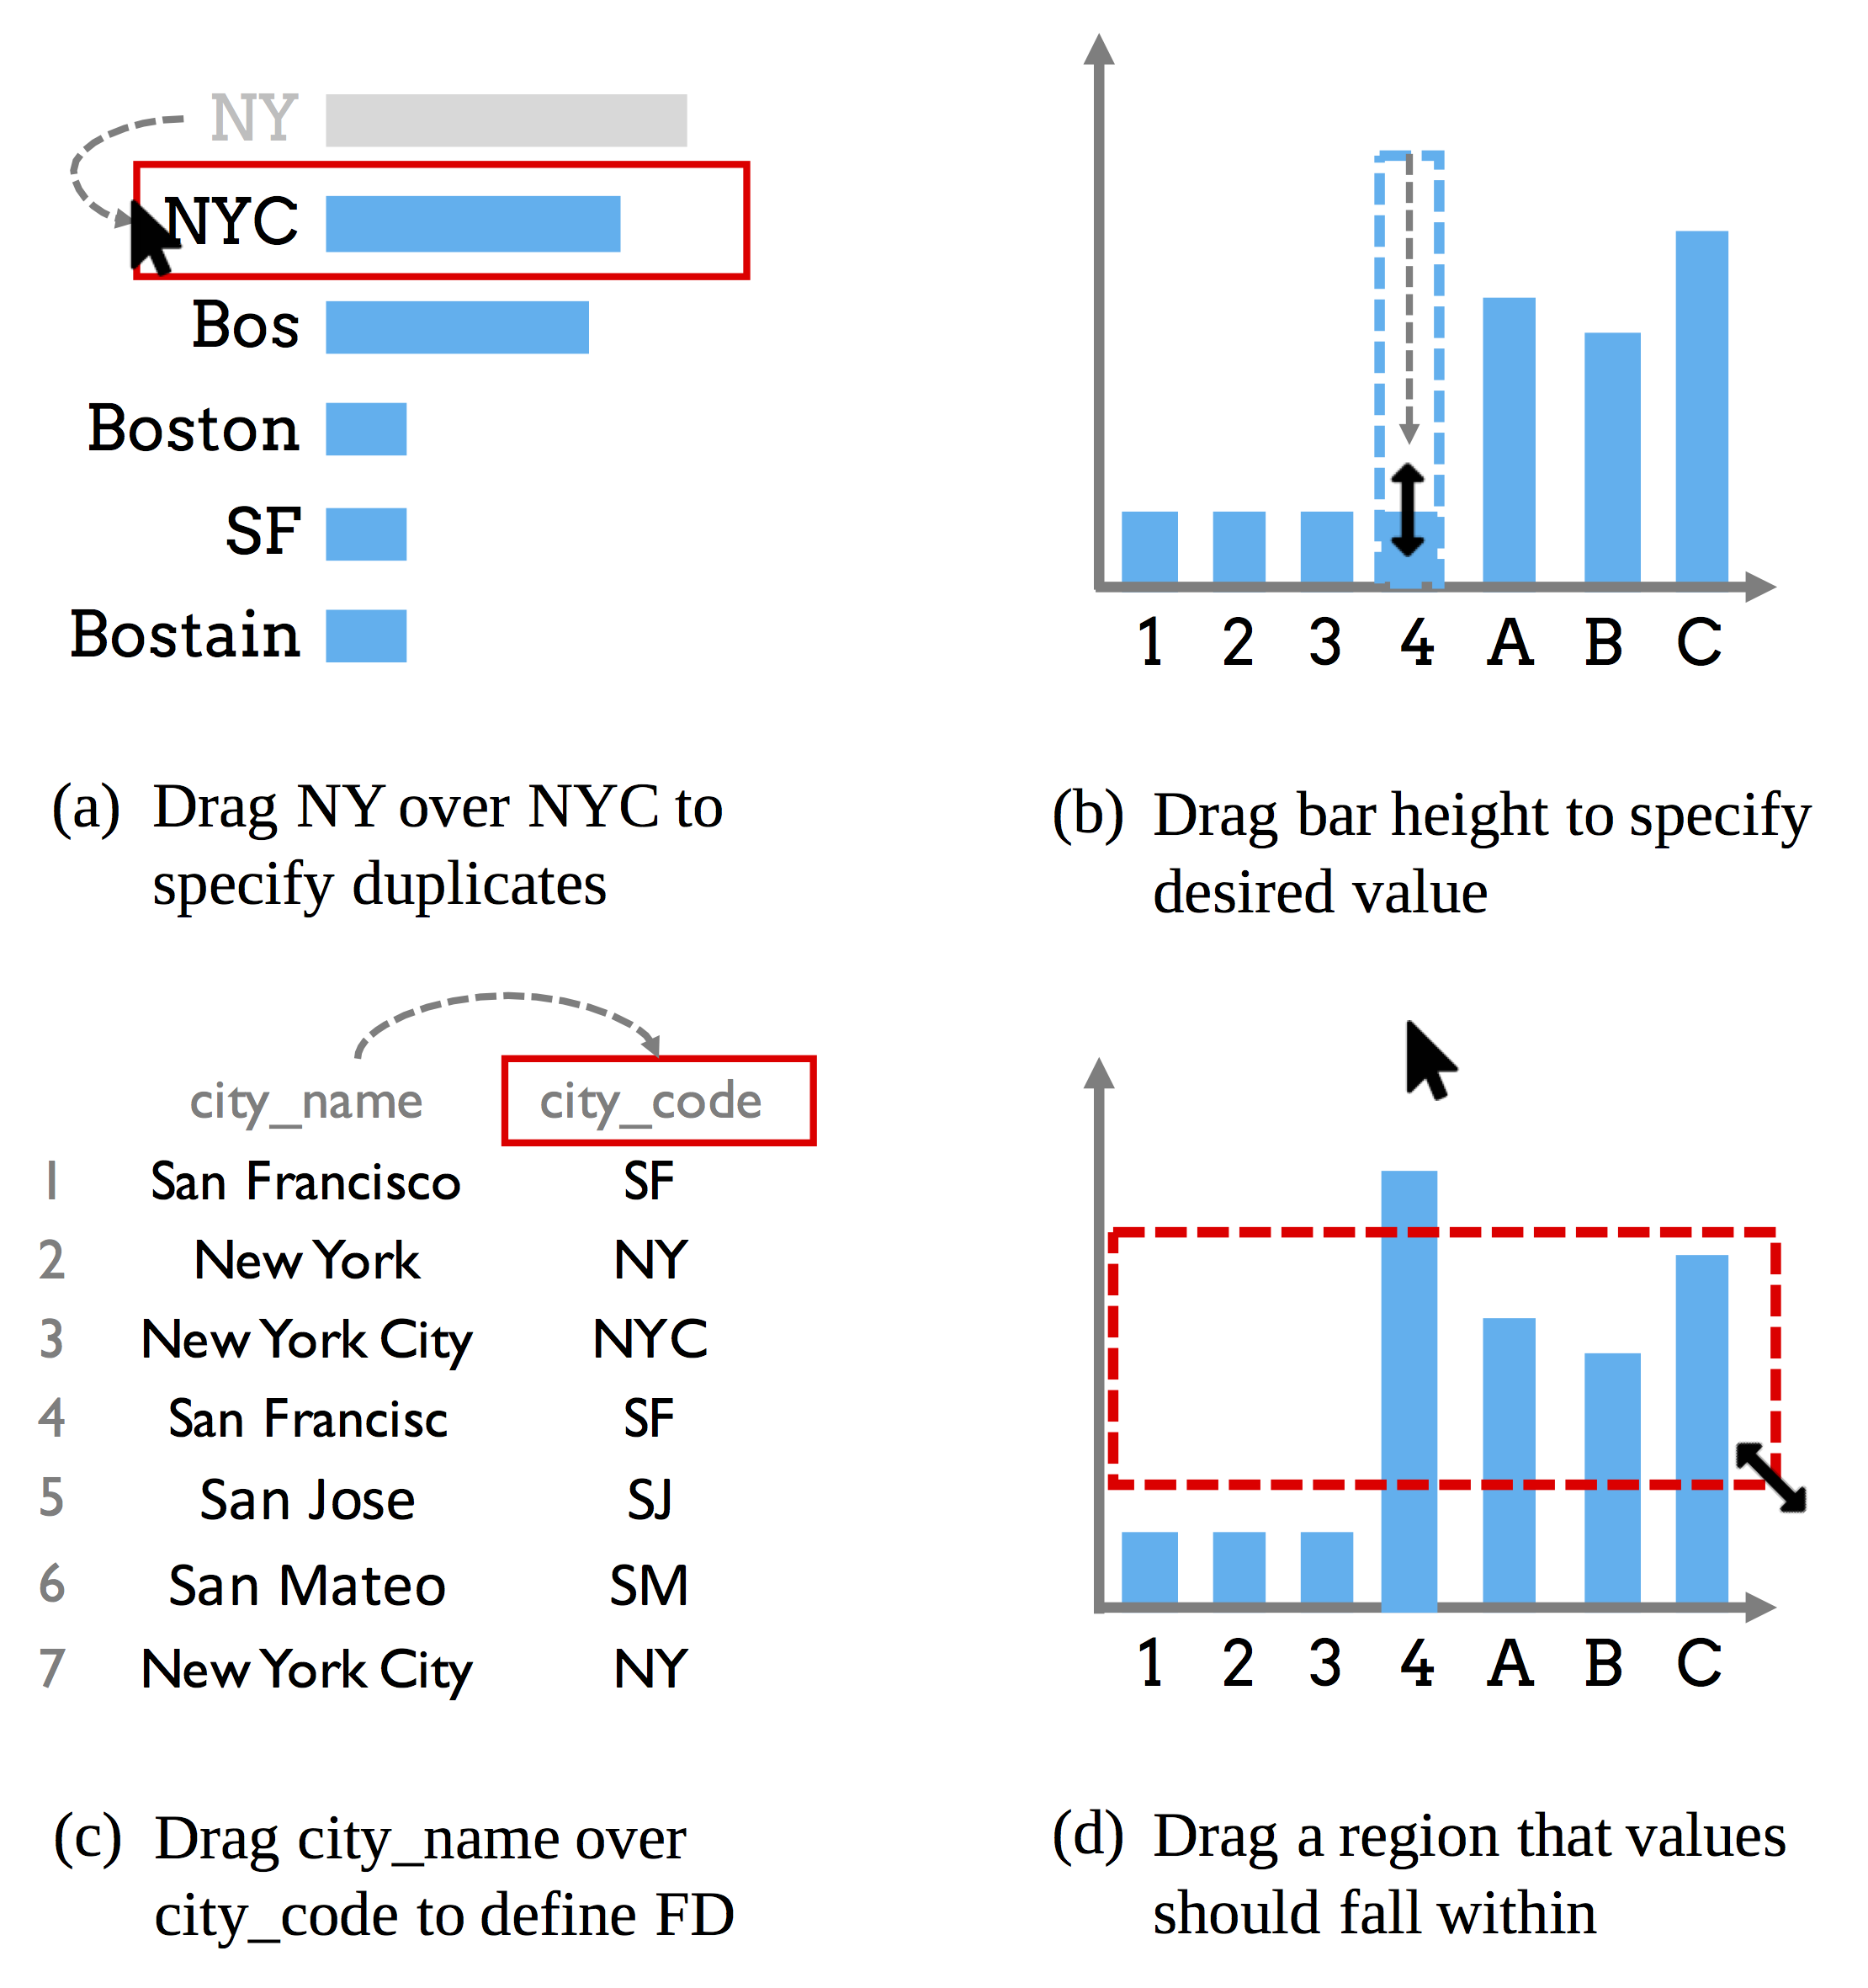
\includegraphics[width=.8\columnwidth]{figures/ui.png}
\label{f:ui}
\caption{Example interactions to specify visualization anomalies. \sys allows a user to specify complaints about a dataset in terms of an arbitrary scoring function and then searches over a language of transformations to best explain those complaints (i.e., what transformations remove them).}
\end{figure}

Going back to the terrorism dataset example, one key limitation of existing explanation engines is that they often only provide a partial explanation for why an aggregate is erroneous if there is dirty data in the mix. Predicate deletion may not be enough to explain output anomalies and may return a trivial or misleading result when there are errors. In Example~\ref{e:terrorism}, the dataset contains three classes of errors:  duplicates, zero-encoding rather than NULLs, and inconsistencies in location attributes. Rather than predicates that are \emph{correlated} with these anomalies, one would like to know suggested transformations that might make an anomalous aggregate typical--including setting values to defaults, merging entities, etc. 

An ideal explanation interface would allow the user to interactively specify the anomalies within the visualization that presented the anomalies, and allow an {\it explanation engine} to generate explanations in the form of succinct sequences of data transformations selected from an extensible library. Furthermore, it should be independent of the visual interface and detection model; effectively allowing for black box complaint specifications.

As a step towards this vision,  we present \sys, a transformation-oriented explanation engine that generalizes prior explanation engines along three dimensions---analysis program, anomaly types, and explanation language. 
\sys  provides a general API to generate explanations in the form of high-level transformation sequences for a wide range of anomalies that can be detected in an output visualization. Transformations are generated from an extensible library of parametrized data transformations.
Formally, \sys takes as input a {\it quality function} that scores each output record as a real-value between $[0,1]$ and a {\it language} of parameterized data transformation operators, and uses a search-based algorithm to output a sequence of transformations (an explanation) from the language that seeks to maximize the quality function.  Similar to prior work~\cite{scorpion}, the quality functions can be derived from interactions in a visualization interface. For example, one can generate a threshold rule that determines anomalous years in the terrorism dataset.  This API imposes minimal restrictions on the quality function, giving it tremendous flexibility regarding the data errors that it can express.   

The primary technical challenge is to quickly search the space of possible explanations.  This space is combinatorial in the possible transformation sequences as well as the possible parameterizations for each transformation in the sequence.  
To address this challenge, we make two key observations: 1) most errors are systematic in nature and their structure can be leveraged to reduce the search space, and 2) explanation generation can be cast as a planning problem, where the quality function is the objective and the explanation is the plan,  and leverage recent advances in robotics and reinforcement learning~\cite{dpm}.


\sys uses a best-first search that greedily appends data transformations to a set of best candidate programs seen so far, and adopts parallelization and pruning ideas from the search-based planning literature.  
In contrast to traditional search problems, where the search state (e.g., chess board) is compact and largely trivial to parallelize in a distributed setting, the data cleaning search state is the size of the input dataset and introduces a trade-off between communication costs to share intermediate state and the degree of parallelism possible.  
 To further accelerate its runtime, \sys can also encode problem-specific optimizations as search pruning rules (e.g., disallowed transformation sequences) or modifications to the data representation (e.g., clustering similar records).  
\sys also leverages the structure of systematic errors to adaptively learn prune rules during the search process, and estimate where or not candidate search branches will ultimately result in high-quality transformation sequences.  
 
The purpose of our experiments is to show the feasibility of a general search-based approach to explanation generation on real-world datasets and analyses.  To this end, we evaluate \sys on 8 real-world datasets used in prior data explanation and data cleaning literature. In each of these uses cases, we present different classes of quality functions and transformation languages--show that \sys is sufficiently general to address all of the domain specific challenges. 
In addition, we use synthetic datasets and errors to evaluate the precision, recall, and complexity of our proposed explanations in a controlled environment.  
We quantitatively evaluate \sys on its ability to generate accurate transformation rules in terms of accuracy on 7 real case studies. We create best effort pipelines for these case studies with existing systems and compare accuracies and runtimes.

% \sys certainly overlaps with data cleaning systems so we present comparisons when relevant.








\if{0}
\ewu{SANYAS TEXT BELOW}


% Detecting and handling dirty data is one of the most time-consuming steps of the data analysis process~\cite{nytimes}.
% It is often the case that such data is first identified by analysts during exploratory data analysis through visualizations or summary statistics that contain anomalous or otherwise unexpected values.

Predicates alone may not adequately explain all types of data anomalies.
Consider a dataset where both \texttt{New York} and \texttt{New York City} refer to the same \texttt{City} entity.
An analyst might detect an anomaly where a count aggregate is unexpectedly low for the group \texttt{New York}. 
A predicate explanation indicates that there exists a predicate, for example, \texttt{City = ``New York''}, that selects all of the anomalous values. 
However, this is only partial information--it tells the analyst nothing about the presence of the alternate entity \texttt{New York City}. 

In general, syntactic errors in a dataset are inherrently explained by data transformations--not just predicates.
It is desirable for the explanation engine to return a complete mapping rule, such as  \texttt{New York} $\rightarrow$ \texttt{New York City}, instead of just the predicate.
We can define a \emph{transformative explanation} as a minimal sequence of such rules from a formal language of rules such that after transformation the flagged values are no longer anomalous. 
Predicate explanations are a special-case of this framework, where the transformation rules are only deletions--in other words, identifying predicates to exclude from base data to remove a group of anomalous values.

\fi

% 
% It is widely known that data cleaning is one of the most time-consuming steps of the data analysis process~\cite{nytimes}, and
% designing algorithms and systems to automate or partially automate data cleaning continues to be an active area of research~\cite{DBLP:conf/sigmod/ChuIKW16}.
% Automation in data cleaning is challenging because real-world data is highly variable. 
% A single data set can have many different types of data corruption such as statistical outliers, constraint violations, and duplicates.
% Once an error is detected, there is a further question of how to repair this error, which often depends on how the data will be used in the future.
% 
% This variability creates a tension between generality and efficiency.
% While one might want a single cleaning framework that addresses all types of errors and repair operations, it is far more efficient to consider more specialized frameworks.
% Data cleaning tools are often highly optimized for particular problems  (e.g., see statistical outliers~\cite{hellerstein2008quantitative}, enforcing logical constraints~\cite{DBLP:conf/sigmod/ChuIKW16}, entity resolution~\cite{DBLP:journals/pvldb/KopckeTR10}). 
% Consequently, a recent survey of industry suggests that data cleaning pipelines are often a patchwork of custom scripts and multiple specialized systems~\cite{krishnan2016hilda}.
% The overhead to setup, learn, and manage multiple cleaning systems can easily outweigh the benefits.
% Some data scientists eschew automated tools altogether and simply write data cleaning programs from scratch.
% The customized programming approach quickly becomes difficult to mantain and interpret; especially for users without data engineering expertise~\cite{sculley2014machine}.
% 
% A single cleaning system that exposes a sufficiently flexible interface is clearly desirable; as long as the runtime and accuracy can be made comparable to existing alternatives.  
% To achieve this, we turn to the contemporary AI literature, which has produced exciting results such as AlphaGo~\cite{silver2016mastering} that were previously considered not possible.    This work shows that a combination of machine learning and massively parallelized search can effectively optimize highly complex objective functions.
% Our main observation is that data cleaning is very similar to the search problems considered in AI~\cite{russell1995modern}.
% The classic application is a computer chess program that must plan a sequence of chess moves that change the state of the board in order to maximize the likelihood of a checkmate. Likewise, in data cleaning, one is given a dirty relation and a way to measure data quality (e.g., number of integrity constraints violated), and the data cleaning problem is to find a sequence of modifications to the relation that maximize the data quality metric.
% 
% Most non-trivial problems are very hard without good search heuristics.
% Advances in machine learning have made it possible to replace hand-crafted heuristics with automatically learned pruning functions that estimate the expected quality of candidate plans. AlphaGo learned pruning heuristics using a neural network trained on data generated through self-play~\cite{silver2016mastering}.
% This insight is highly relevant to data cleaning, where datasets tend to have structure amenable to learning heuristics adaptively.
% Data errors are often systematic where they are correlated with with certain attributes and values in the dataset~\cite{rekatsinas2017holoclean,DBLP:journals/pvldb/KrishnanWWFG16}.
% Consequently, as more data is cleaned, we can better identify common patterns to prioritize the search on future data.
% We may not necessarily need a neural network for data cleaning, but the overall algorithmic structure of AlphaGo, tree-search combined with a learned heuristic, can be very useful.
% 
% \sys is a new data cleaning system that is designed around a search-based model. It takes as input a {\it quality function} that models the data quality of a relation as a real-value between $[0,1]$ and a {\it language} of parameterized data cleaning operators, and outputs a sequence of data cleaning transformations (a cleaning program) from the language that seeks to maximize the quality function.This API imposes minimal restrictions on the quality function, giving it tremendous flexibility in terms of the data errors that it can express.   As a comparison, a recent system called Holoclean~\cite{rekatsinas2017holoclean} is similar in that it provides a rich interface to specify denial constraints and lookup tables, and integrates them within a probabilistic model to more accurately resolve constraint violations.  In contrast, \sys's quality function is a user-defined function that can express {\it arbitrary combinations} of denial constraints {\it as well as} statistical, quantitative, text formatting, and other classes of data errors.  For instance, \Cref{s:expquant} shows how \sys can perform cleaning for machine learning applications by embedding machine learning training and evaluation within the quality function, while \Cref{s:expterror} combines entity resolution, outlier cleaning, and functional dependency violations within the same function.  
% 
% 
% \sys uses a best-first search that greedily appends data transformations to the set of best candidate programs seen so far, and adopts parallelization and pruning ideas from the search-based planning literature.  In contrast to traditional search problems, where the search state (e.g., chess board) is compact and largely trivial to parallelize in a distributed setting, the data cleaning search state is the size of the input dataset and introduces a trade-off between communication costs to share intermediate state and the degree of parallelism possible.  
% To further accelerate its runtime, \sys can also encode problem-specific optimizations as search pruning rules (e.g., disallowed transformation sequences) or modifications to the data representation (e.g., clustering similar records).  We find that many optimizations in existing cleaning systems may be cast as search pruning rules.
% 
% \sys can adaptively learn pruning rules to avoid unprofitable search branches during the search process.
% While AlphaGo used a deep neural network and massive amounts of training data to model the heurisitic, we found that a simple logistic regression classifier and training data gathered during the search process was sufficient to reduce the runtime by multiple orders of magnitude. 
% It is important to acknowledge that \sys loses many of the provable guarantees provided by specialized systems based on logical constraints, and is in some sense, best-effort.  
% Across 8 real-world datasets used in prior data cleaning literature, we show that \sys matches or exceeds the cleaning accuracy and exhibits competitive run-times to state-of-the-art approaches that are specialized to a specific error domain (constraint, statistical, or quantitative errors).  
% 
% \subsection{Main Benefits}
% \begin{itemize}[leftmargin=*, topsep=0mm, itemsep=0mm]
% \item \stitle{Optimization} Existing cleaning pipelines must combine disparate cleaning solutions and manage glue code to transfer data between systems.  However, data transfer can be a non-trivial portion of the total cleaning cost and recent work~\cite{palkar2017weld} has shown that a common runtime can avoid data movement and improve runtimes by up to $30\times$.  
% 
% \item \stitle{Generalization and Robustness} In contrast to existing cleaning systems, that output a cleaning relation, \sys outputs a composable cleaning program that is both simpler to understand because it groups common fixes together, and can be applied to new data.  In addition, the cleaning program allows us to analyze cleaning systems for overfitting.  We indeed find that the complexity of the quality function and cleaning language can lead to overfitting, and believe this is the case for any data cleaning system.  We also show that simple changes to the quality function can act as regularization terms to control the degree of overfitting.
% 
% \item \stitle{Software Engineering}  Users do not need to write and manage glue code; do not need to manage ETL between systems; and do not need to learn system specific abstractions, languages, and assumptions.  All of these are arguably intangible, but critical friction points in the highly iterative cleaning process.  
% 
% \item \stitle{New Cleaning Applications} We envision that a single API makes it possible to support an ecosystem of domain-specific cleaning specification libraries.  For instance,  interactive visualization interfaces akin to~\cite{trifacta,kandel2011wrangler,DBLP:journals/pvldb/0002M13,wu2012demonstration} can directly translate user interactions into a wide range of cleaning constraints.   
% \end{itemize}
% 
% 
% 
% 
% % * single library/language with the same abstraction is important (software engineering)
% %   * no more glue code -- talk about weld, etc.  
% %   * no ETL between systems
% %   * no leraning new abstractions
% %   * new languages to specify constraints and quality goals.  some are languages, some are APis, some are systems
% %   * engineering: systems like llunatic, need to satisfy postgres schema to get started
% % 
% % * different
% %   * application driven cleaning by embedding downstream app into the quality function
% %   * new apps
% %     * viz stuff needs a single api
% %     * mixed datasets -- numeric and relational data
% %     * many interfaces to compose and create quality functions and languages
% % 
% % * holoclean
% %   * lets them express denial constraints and use a knowledge base to decide how to resolve violations
% %   * we suppor denial constraints, as well as numeric errors, text extraction errors, and arbitrary formulations of teh quality measure.  
% % 
% % 
% % * unification -->
% %   * reduces engineering to implement cleaning system
% %   * joint optimization if overlapping in 
% % * generalize to new data 
% %   * overfitting
% % * parallelize opportunities
% 
% 
% 
% 
% 
% 
% 
% 
% 
% 
% 
% 
% \if{0}
% Data cleaning usually involves tedious manual specification of transformation rules.
% For example, a data scientist might write a rule that maps every record with a \textsf{country} attribute ``United States'' to ``United States of America''.
% These collections of rules quickly grow in size, and if they are developed in an ad-hoc way, they can be brittle and hard to maintain~\cite{krishnan2016hilda}.
% Overly specific rules may not apply to future data, and overly general rules, might introduce unwanted side-effects.
% Designing accurate transformation rules is a painstaking process, which is widely reported to be one of the most effort-intensive steps in data science~\cite{nytimes}.
% 
% We explore to what extent such transformation rules can be learned through a process of automatic trial-and-error on a dataset.
% The system simulates different sequences of data transformations and scores the result according to a user-specified data quality objective function.
% On its own, this is an inefficient way to search to search the set of transformation rules.
% However, we can leverage Machine Learning to learn a strong pruning heuristic incrementally.
% Transformations are often parametrized by literal values from the database (e.g., find string X and replace with string Y).
% If we clean data in small partitioned blocks, we can incrementally build a classifier that infers common patterns in these literals, such as whether the strings tend to be similar or tend to be different or the attributes that are likely to be touched.
% For example, consider the problem above where a data scientist is resolving inconsistencies in a \textsf{country} attribute to satisfy an integrity constraint.
% As we iterate through the distinct \textsf{country} values and simulate possible replacement values, it might become clear that the source string have to be close to the target strings in string similarity, i.e., ``United States'' is more likely to be replaced by ``United States of America'' than ``Zimbabwe''.
% Learning such a relationship automatically avoids hand coded heuristics which have to consider the complex relationship between how the analyst describes data quality and how exactly the transformations are defined.
% 
% This basic algorithm, optimizing a sequence of black-box transformations over a black-box data quality function, has a number of important advantages: (1) it is highly expressive as it can model a wide range of data cleaning formalisms from integrity constraints to quantitative data cleaning in the same framework, (2) it is relatively easy to parallelize the search, and (3) the result of the algorithm is not only a cleaned database instance but transformations that can be applied to future data.
% This formalism casts data cleaning as a planning problem; analogous to the algorithms used AI, Robotic Planning, and Control.
% Similar to the way one plans out a sequence of chess moves in AI to gain a strategic board position, we can think of data cleaning as planning out a sequence of data transformations to maximize the score on a data quality function.
% And as in chess, where one cannot perfectly anticipate the opposing player's moves, in data cleaning we may not have a strong \emph{a priori} model of how a user-defined transformation rule modifies the data.
% As a result, the algorithm and search heuristics cannot make strong assumptions about the anticipated structure of any search instance.
% This sort of an approach is increasingly attractive because recent results in AI demonstrate scaling these search problems to  high branching-factor domains even when few assumptions are made.
% Recent algorithms have been shown to match or exceed human performance in domains such as Go~\cite{silver2016mastering} and in Atari video games~\cite{mnih2015human}.
% As in many classical data cleaning problems, an optimal solution to AI search problems is very hard to discover, but pragmatically leverage distributed computing and pruning rules learned from data can tractably find acceptable solutions.
% 
% We use this algorithm as a starting point for a new data cleaning system called \sys.
% We designed an API that takes classical data cleaning problem specifications, such as integrity constraints, gold-standard manually cleaned data, and statistical models, and translates those specifications into an iterative learning search problem. 
% Of course, we often need special-case optimizations that prune unproductive search branches to make the runtime more competitive with special case systems.
% We provide a model where pruning rules are specified as regular expressions over a formal language of transformations and can be static (i.e., fixed before execution) and dynamic (i.e., inferred from properties of the dirty database instance).
% The search algorithm we use is a memory-bounded best-first search which maintains the subset of the search frontier that can fit in memory. 
% This algorithm can be parallelized, distributed, and can cache repeated computations.
% \fi
% 
% 
% 
% \if{0}
% 
% 
% view data cleaning from a planning~\cite{} and optimization perspective, and show evidence that a simple, general approach to this problem can provide the user with considerable flexibility in terms of cleaning data with different classes of errors, controlling the allowable operations, and customizing the system to new types of data errors.
% 
% 
% 
% Ideally, the majority of the data cleaning process should reside in a single system with a  \emph{declarative} interface, wherein the analyst specifies a high-level data model (e.g., constraints the data should satisfy) and a system automatically generates the pipeline to enforce the model.
% The idea of declarative data cleaning is not new~\cite{rahm2000data}, but such approaches have classically been restricted to data models specified in subsets of first-order logic and only recently have considered extensions better handle uncertain numerical data~\cite{prokoshyna2015combining}.
% The prevailing wisdom is that there is an inherent tradeoff between the expressiveness of the data model and the efficiency of the (approximate) solution algorithm---limited models allow the system designer to exploit specific algorithmic structures.
% 
% 
% However, two recent trends, namely, the success of model-free learning in AI and the availability commodity cloud computing encourage us to reconsider this algorithmic philosophy.
% Recent progress in planning problems such as AlphaGo~\cite{silver2016mastering} and automatically playing Atari video games~\cite{mnih2015human} have shown that a prudent combination of Machine Learning and distributed search can approximately optimize very complex black-box objective functions.
% The intriguing aspect of these results is that the same algorithm, called Deep Q Reinforcement Learning, that learns to play an Atari game~\cite{mnih2015human} can be used on a very different problem, such as training a robot~\cite{gu2017deep}.
% The underlying optimization algorithm encodes few specifics about the objective or structure of the domain  and pragmatically finds a reasonable local optimum.
% The optimization algorithm is general enough to support a very wide class of problems--at the cost of additional computational resources since it is unaware of instance-specific structure.
% 
% \fi
